\documentclass[a4paper]{article}

\usepackage{amsmath}
\usepackage{amssymb}
\usepackage{parskip}
\usepackage{fullpage}
\usepackage{hyperref}
\usepackage{chronology}
\usepackage{stellar}
\usepackage{bettelini}
\usepackage{tikz}
\usepackage{fancybox}
\usepackage{makecell}

\usetikzlibrary{cd}

\hypersetup{
    colorlinks=true,
    linkcolor=black,
    urlcolor=blue,
    pdftitle={Geografia},
    pdfpagemode=FullScreen,
}

\title{Geografia}
\author{Paolo Bettelini}
\date{}

\begin{document}

\maketitle
\tableofcontents
\pagebreak

\part{Geografia Economica}

\section{Esercizio: la Francia ferita nell'epoca delle policrisi, Edgar Morin}

\textbf{Identifica e sintetizza in una linea del tempo i principali riferimemti storici}

\begin{chronology}[25]{1789}{2023}{\textwidth}
    \event{1789}{Rivoluzione Francese (1789)}
    \event{1830}{Rivoluzioni e crisi (1830-1906)}
    \event{1901}{Multiculturalismo francese (1901)}
    \event{1914}{Prima guerra mondiale (1901)}
    \event{1929}{Crisi economia (1929)}
    \event{1939}{Seconda guerra mondiale (1939)}
    \event{1947}{Guerra Fredda (1947)}
    \event{1956}{Crisi del comunismo (1956)}
    \event{1968}{Rivolta studentesca (1968)}
    \event{1974}{National Rally (1972)} % cambiato anno per non sovrascrivere
    \event{1989}{Caduta Muro Berlino (1989)}
    \event{2014}{Guerra Russo-Ucrania (2014)}
\end{chronology}

\textbf{Identifica i riferimenti spaziali e specifica quali sono le scale geografiche mobilitate dall'autore}

L'autore cita riferimenti spaziali su tre diverse scale geografiche.
Vengono citate per la scala nazionale nazioni con grandi influenze politiche, quali la Francia,
Russia e Stati Uniti.
Vengono citate l'Europa, Africa o l'Occidente.
Come scala più ampia viene citata quella globale.

\textbf{Definisci brevemente il termine "policrisi" spiegando l'evoluzione del concetto}

\sdefinition{Policrisi}{
    Una \textit{policrisi} è un insieme di molteplici event nefasti e interdipendenti che potrebbero
    portare a danni su grande scala (planetaria).
}

La "policrisi" sottolinea l'idea che il mondo moderno sia
caratterizzato da una profonda interconnettività.

\textbf{Proponi una riflessione argomentata sui contenuti delle ultime 4 righe del testo}

Evitare che la Francia (la Repubblica) si trasformi in uno stato del controllo
è uno degli step fondamentali per ridurre la policrisi,
essendo la Francia un importante tassello della policrisi globale.

\textbf{Riassumi in due (o tre) frasi il contenuto del testo}

Le relazioni fra eventi di scale diverse, sia a livello locale che a quello globale, 
sono interdipendenti e portano a situazioni di crisi globali.

Eventi che sono all'apparenza locali possono avere grandi effetti in crisi di scala maggiore.

\pagebreak

\section{Secolo}

\sdefinition{Secolo}{
    Un \textit{secolo} può essere definito in mainera stretta come 100 anni,
    oppure come un periodo di circa 100 anni con caratteristiche omogenee.
}

\section{USA vs URSS}

\sdefinition{NATO}{
    La \textit{NATO} (North Atlantic Treaty Organization) è un associazione di sicurezza composta dsa diverse nazioni.
}

\begin{center}
    \begin{tikzcd}
        \fbox{\textbf{USA}}               & \textit{differenze}                       & \fbox{\textbf{URSS}}               \\
        \text{Democrazia}          & \ovalbox{\textbf{Politiche}} \arrow[r] \arrow[l]  & \text{Autocrazia}           \\
        \text{Economia di mercato} & \ovalbox{\textbf{Economiche}} \arrow[r] \arrow[l] & \text{Economia pianificata} \\
        \text{NATO}                & \ovalbox{\textbf{Militari}} \arrow[r] \arrow[l]   & \text{Patto di Varsavia}   
    \end{tikzcd}
\end{center}

% https://moodle.edu.ti.ch/libe/pluginfile.php/114669/mod_resource/content/0/Presentazione%20Secolo%20breve.pdf

% https://moodle.edu.ti.ch/libe/pluginfile.php/114664/mod_folder/content/0/1Viola%20-%20La%20crisi%20del%2029.pdf?forcedownload=1

% TODO L’ascesa dell’ordine economico globale
% espandere commercio internazinoale
% regole vincolanti
% sistema stabile dei cambi
% 3 organi internazinoali: banca mondiale, FMI, GATT (-> WTF 1995)

% I 30 gloriosi
% --- Caratteristiche
% Welfare state, stato sociale esteso
% meno disoccupazione più posti lavoro
% forte crescita econimica
% --- Ragioni / Cause
% Ricostruzione
% I nuovi accordi sul commercio mondiale
% La stabilità del sistema economico
% ________

\pagebreak

\part{Geografia Fisica}

\section{L'interazione tra le sfere terrestri}

La terra può essere suddivisa in diverse sfere interdipendenti.

\sdefinition{Atmosfera}{
    Componente gassosa che avvolge il pianeta. L'aria è inodore e incolore ed è quasi 800 volte meno densa dell'acqua.
}

\sdefinition{Idrosfera}{
    Insieme di tutte le acque del pianeta nei diversi stati di aggregazione; comprende le acque marine e quelle continentali.
}
    
\sdefinition{Litosfera}{
    Componente solida superficiale costituita dalle rocce.
}

\sdefinition{Biosfera}{
    Componente vivente e comprende gli organismi che popolano la zona di interazione delle tre sfere precedenti.
}

% TODO Astenosfera

% https://tikzcd.yichuanshen.de/#N4Igdg9gJgpgziAXAbVABwnAlgFyxMJZARgBpiBdUkANwEMAbAVxiRAB12cYAPHYAEL44AMxgAnOgF8QU0uky58hFGQAMVWoxZtO3PsACCOALaYxkmXIXY8BIgCZSDzfWatEHLr34AZXOYS0rLyIBi2ykRqzq7aHl76-ACSUOKBlrKaMFAA5vBEoCJpJkhkIDgQSE4gAEYwYFBIAMxq1iBFECWIZRXN1HUNSAC0LW0dXU3UvYjVA42II62h40jR5ZXd-fXzo8vFpVMba3PNS4X7M4d9tdvDu+ed19PHtwv37Rdr05M3g29nH0eiC+G1mr3eK0u61WWz+EIu1WmZROCwALABOMYXH5I2HzDHUBhYMDxOAQImNagACxgdHmYCYDAYUzoWAYbEgJMyUiAA
%\begin{tikzcd}
%    & \text{Atmosfera} \arrow[rdd, bend left] \arrow[ldd, bend right] \arrow[d, bend left] &                                                                                          \\
%    & \text{Biosfera} \arrow[u, bend left] \arrow[ld, bend right] \arrow[rd, bend left]    &                                                                                          \\
%\text{Idrosfera} \arrow[rr, bend right] \arrow[ru, bend right] \arrow[ruu, bend left=49] &                                                                                      & \text{Litosfera} \arrow[ll, bend right] \arrow[lu, bend left] \arrow[luu, bend right=49]
%\end{tikzcd}

I processi che coinvologno le sfere terrestri sono di due tipi:

\sdefinition{Processo Esogeno}{
    Sono processi attivati dall'energia del Sole e avvengono sulla superficie terrestre; sono per esempio i movimento delle acquem, i passaggi di stato, il tempo atmosferi o il modellamento della superficie terrestre.
}

\sdefinition{Processo Endogeno}{
    Sono processi attivati dal calore interno della Terra; sono i processi chde portano alla formazione di catene montuose e di nuovi oceani.
}

\section{Moti convettivi}

\sdefinition{Moto convettivo}{
    I \textit{moti convettivi} sono dei lenti movimenti di materiali solidi.
}

I moti convettivi possono scendere o salire.
Quando i moti salgono e colpiscono la litosfera intaccano le placche tettoniche

\begin{center}
    \bgroup{}
    \def\arraystretch{1.25}
    \begin{tabular}{ |c|c|c|c| }
        \hline
        & \textbf{Direzione scorrimento} & \textbf{\makecell[c]{Forme morfologiche che \\ si originano}} & \textbf{Esempi luoghi} \\
        \hline
        \textbf{Margini divergenti} & Direzioni opposte & Rift Valley & Dorsale medio atlantica \\
        \hline
        \textbf{Margini convergenti} & Direzioni convergenti & XX & XX \\
        \hline
        \textbf{Margini trasformi} & XX & XX & XX\\
        \hline
    \end{tabular}
    \egroup{}
\end{center}

I tipi possibile di margine sono
\begin{itemize}
    \item Oceanica - Oceanica
    \item Oceanica - Continentale
    \item Continentale - Continentale
\end{itemize}

\subsection{Margini divergenti}

% leggere pag 24+ per tutte le tipologie
\begin{figure}[h]
    \centering
    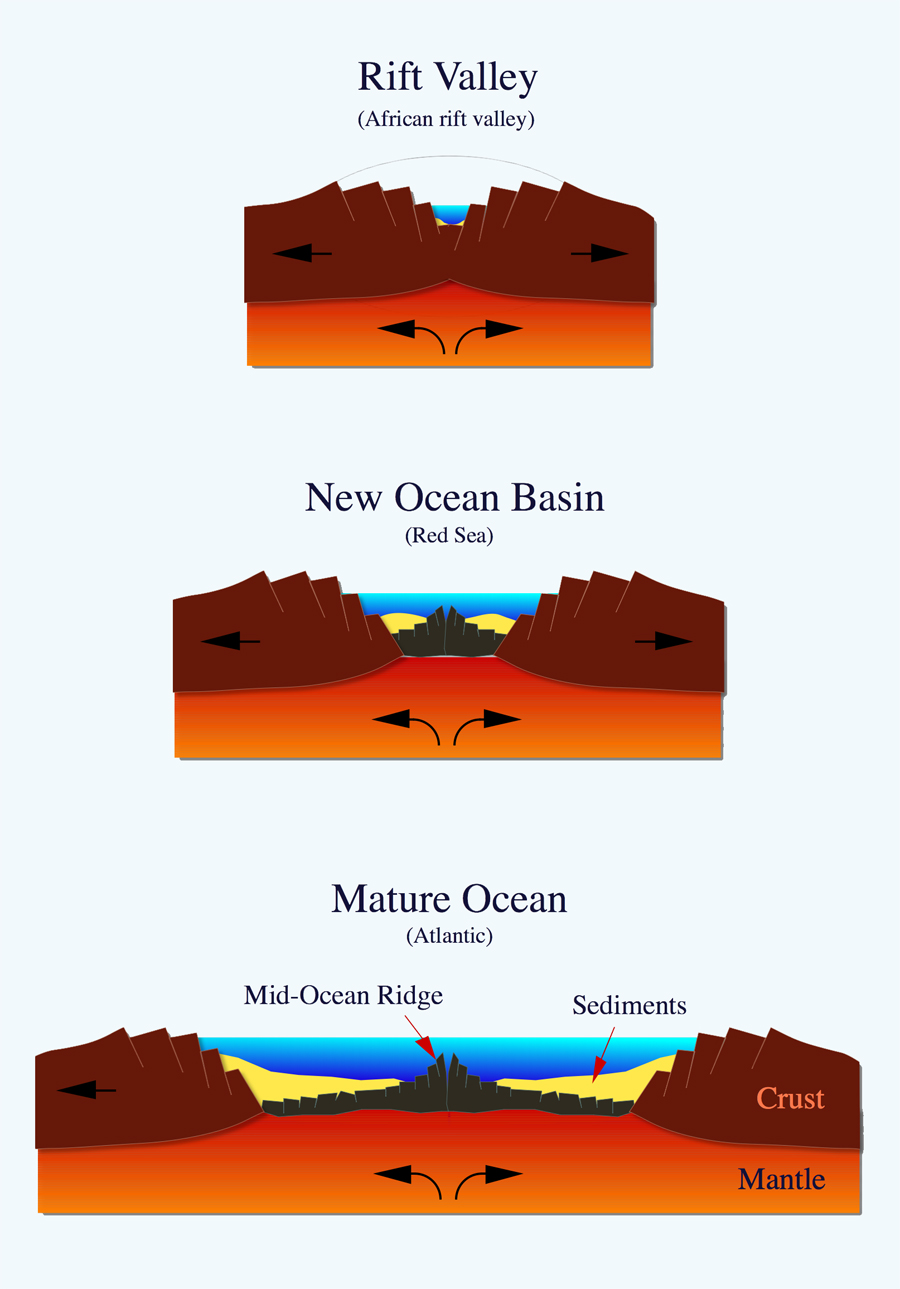
\includegraphics[width=0.5\textwidth]{rift-valley.jpg}
\end{figure}

\pagebreak

\subsection{Margini convergenti}

\begin{figure}[h]
    \centering
    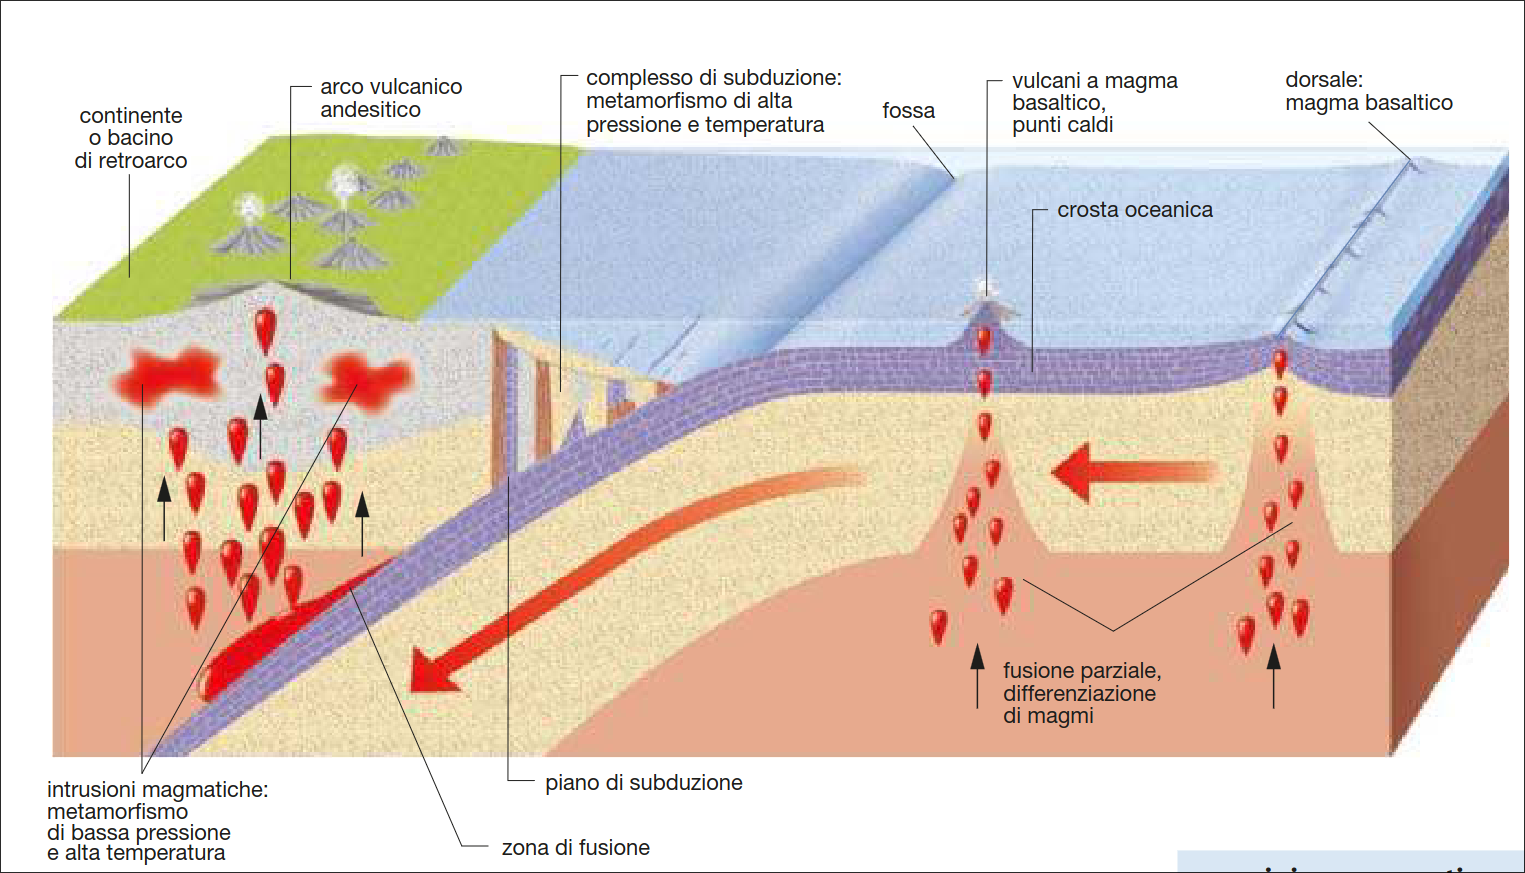
\includegraphics[width=\textwidth]{mconvergenti.png}
\end{figure}

Il materiale che fonde, risale dando origine ad attività vulcaniche.
% Se oceanica-ocdeanica, abbiamo una rcod i isole vulcaniche
% Altrimenti è oceanica-continentale

\end{document}
